\documentclass[10pt,twocolumn,letterpaper]{article}
\usepackage[margin=0.9in]{geometry}
\usepackage{graphicx}
\usepackage{amsmath,amssymb}
\usepackage{booktabs}
\usepackage{xcolor}
\usepackage[colorlinks=true,allcolors=blue]{hyperref}
\usepackage{algorithm}
\usepackage{algpseudocode}
\usepackage{caption}
\graphicspath{{figs/}}
\renewcommand{\ttdefault}{cmtt}
\title{Oracle-Visibility Selective Injection:\\ A Single-View Reconstruction Diagnostic}
\author{Anonymous CVPR submission\\\small Paper ID ****}
\date{}

\begin{document}
\maketitle

\begin{abstract}
Single-view reconstruction is asymmetric: visible regions have image evidence,
whereas disoccluded regions require a prior. We study asymmetric latent injection
as an \emph{oracle-visibility diagnostic}: the released \texttt{visibility.npy}
is produced by running VGGT on the complete target clip and therefore crosses the
single-image inference boundary. The mask leaves the visible latent path exact,
but VAE/decoder spatial mixing prevents a final-RGB guarantee; the direct
16-scene run measured a $+0.016$ dB visible-PSNR change. A target-GT
\emph{quality-gap oracle} correlates with injection benefit at $r=0.982$ over 166
scenes, while always injecting changes from $+2.49$ dB on oracle-hard scenes to
$-2.52$ dB on oracle-easy ones. On a fixed 759-frame component diagnostic, the
always injected output improves Gen3R PSNR from 17.77 to 19.22 dB and LPIPS-VGG
from .360 to .341. Deployment requires a source-only visibility estimator and a
source-observable selector; neither is evaluated here.
\end{abstract}

\begin{figure*}[t]
\centering
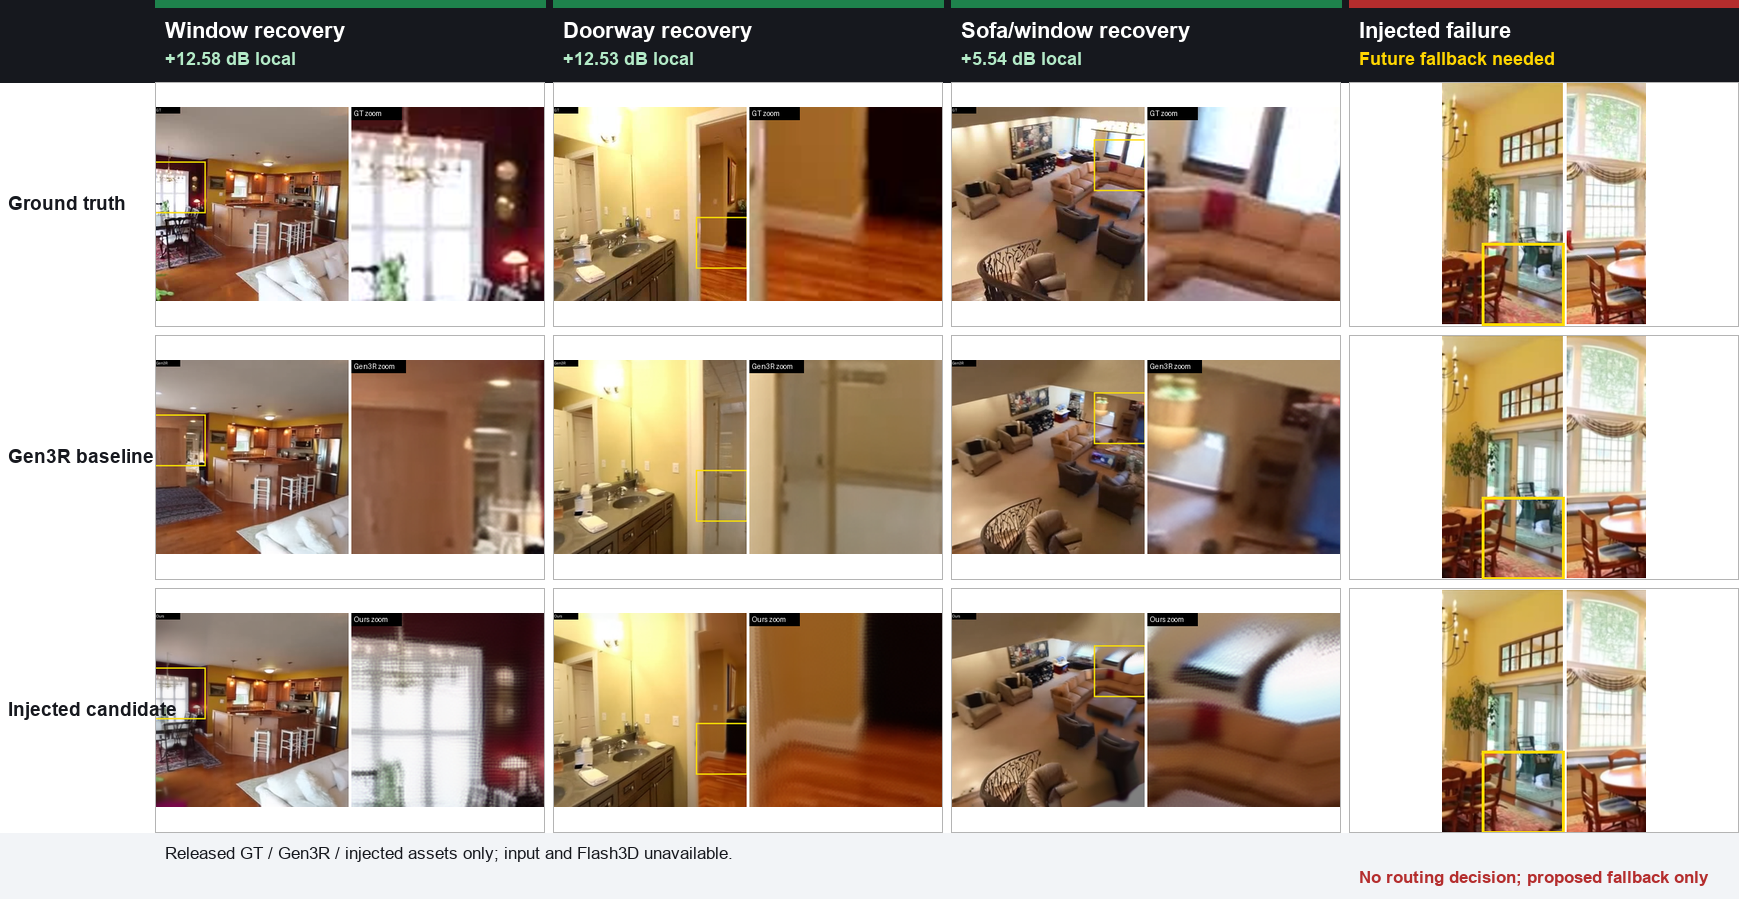
\includegraphics[width=\textwidth]{fig_teaser_aligned.png}
\caption{Released qualitative evidence for the fixed long-sequence diagnostic.
Columns show three successful recoveries (window, doorway/floor, and sofa/window)
and one injection failure. Rows show ground truth, the Gen3R baseline, and the
injected candidate; yellow boxes and adjacent zooms use the same released ROI in
each row. The first three columns report local ROI PSNR gain. The last column
illustrates why a future reliable fallback would be useful; no routing decision is
claimed. The teaser is constrained to released GT/Gen3R/injected assets; missing
input/Flash3D assets are a release limitation, so the approved design uses the
strongest honest teaser available rather than inventing replacements. The figure
supports localized recovery and failure analysis, not an official benchmark comparison.}
\label{fig:teaser}
\end{figure*}

\section{Introduction}
Pixels retained from an input view mainly require geometric transport; pixels
revealed by camera motion have no direct image evidence and must be generated.
Full-image averages obscure this causal distinction. Our central question is:
\emph{when does feed-forward geometric evidence improve a generative
single-view reconstruction, and how can it be injected without harming
already-correct visible regions?}

We treat Flash3D~\cite{flash3d} and Gen3R as components rather than leaderboard
opponents. Flash3D supplies target-aligned geometric evidence, while the frozen
Gen3R backbone supplies a generative prior. A visibility mask routes visible latents around injection exactly. Because
geometric evidence is not uniformly better in disocclusions, we analyze optional
fallback policies, but the released PSNR-based policies require target GT and are
oracle diagnostics rather than deployed model components.

Our three non-overlapping contributions are:
\begin{enumerate}
\item Concept: oracle-visibility selective injection as a mechanism diagnostic, not deployable single-view inference.
\item Mechanism: an exact visible latent bypass, with decoded RGB behavior measured rather than guaranteed.
\item Evidence: a scale-stable quality-gap mechanism and perceptual component gains on a fixed long-sequence diagnostic, bounded by failed zero-shot ACID transfer.
\end{enumerate}

\section{Related Work}
\paragraph{Feed-forward reconstruction.}
pixelSplat~\cite{pixelsplat}, MVSplat~\cite{mvsplat}, and
DepthSplat~\cite{depthsplat} infer Gaussian scenes~\cite{gaussiansplatting} from
two views; Flash3D~\cite{flash3d} addresses one view. We use Flash3D as an
evidence component, not as an official reproduced baseline.
\paragraph{Generative reconstruction.}
ViewCrafter~\cite{viewcrafter}, CAT3D~\cite{cat3d}, and
GenWarp~\cite{genwarp} synthesize unseen content but may drift geometrically. We
retain this prior and condition it only where source evidence is absent.
\paragraph{Selective guidance.}
RePaint~\cite{repaint} conditions known pixels during denoising, while
REPA~\cite{repa} and Geometry Forcing~\cite{geometryforcing} alter training. Our
intervention is test-time, region-asymmetric, and allowed to abstain.

\section{Method}
\begin{figure*}[t]
\centering
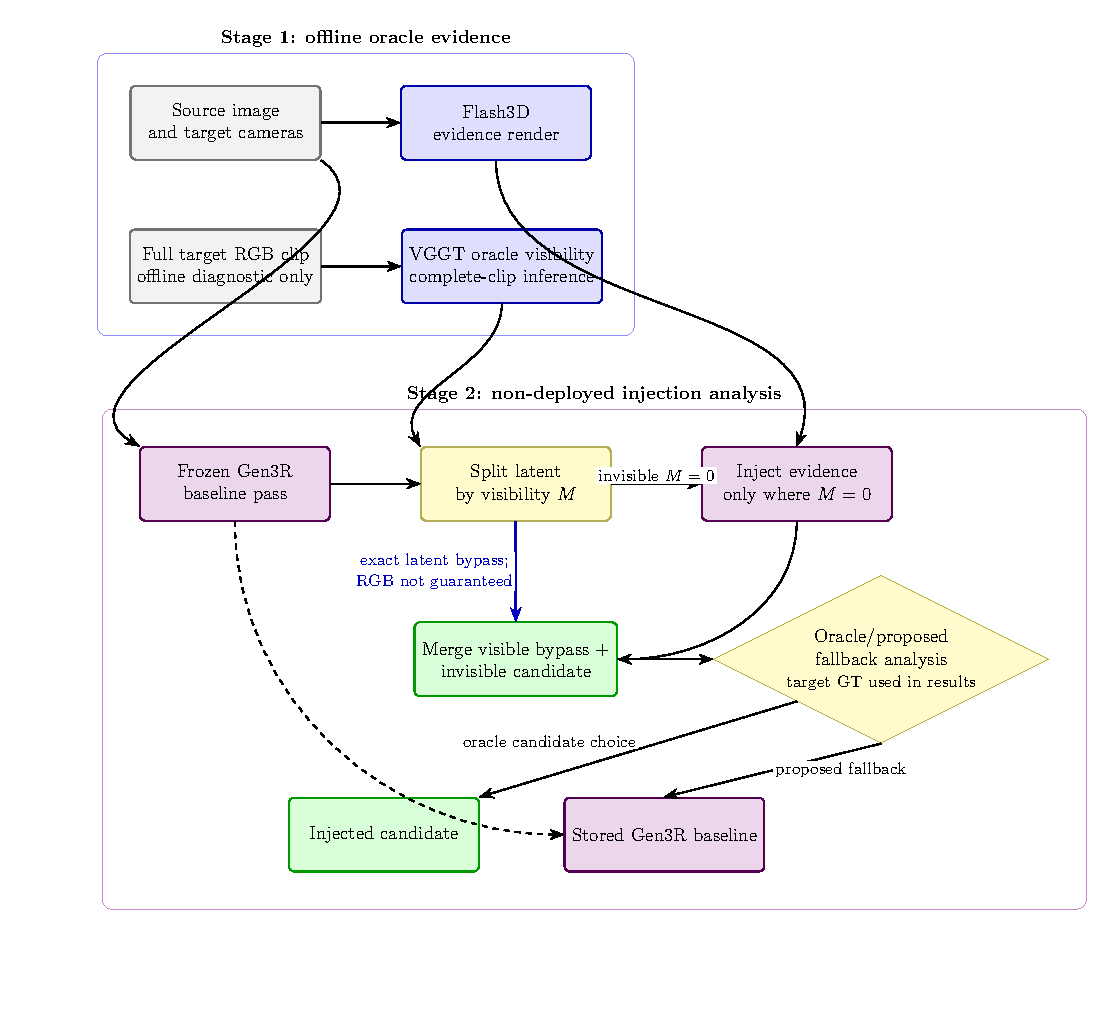
\includegraphics[width=0.9\textwidth]{fig_pipeline.pdf}
\caption{Offline oracle-visibility diagnostic. VGGT processes the complete target
clip to construct $M$, crossing the single-image inference boundary. Stage 2
obtains the frozen Gen3R baseline, preserves the visible latent path exactly, and
injects evidence only into invisible latents. This does not guarantee exact
visible RGB after VAE decoding. The fallback branch is also oracle analysis using
target GT. A deployable method needs source-only visibility and selection
estimators; neither is released or evaluated.}
\label{fig:pipeline}
\end{figure*}

Let $M\in\{0,1\}$ denote oracle visibility ($1$ is visible), $z$ the current
Gen3R RGB latent, $z_{\rm f3d}$ encoded evidence, and $w$ a fixed clean-space
agreement weight. At each denoising step,
\begin{equation}
z'=M\odot z+(1-M)\odot[(1-w)z+wz_{\rm f3d}].
\end{equation}
For $M=1$, $z'=z$ exactly on the masked latent path. We compute $w$ in clean
latent space from agreement between evidence and the baseline. Because the VAE
and decoder mix spatial neighborhoods, the equation does not prove final visible
RGB invariance; the direct 16-scene run measured $+0.016$ dB visible-PSNR change.
For analysis only, the \emph{visible-quality proxy}
$\mathrm{PSNR}_{\rm f3d,vis}-\mathrm{PSNR}_{\rm base,vis}$ probes relative
visible-region quality against target GT; despite using the visible region, it is
not available at raw test time. The only released scene-level quantity independent
of target GT is VGGT's \texttt{vis\_frac}, whose local policy was weak and is not
a main result.

\begin{algorithm}[t]
\caption{Asymmetric geometry-guided generation}
\begin{algorithmic}[1]
\State \textbf{Input:} image $I$, target poses $P_t$, masks $M_t$
\State $z_{\rm f3d}\gets\mathrm{Encode}(\mathrm{Flash3D}(I,P_t))$
\State $z\gets G(I,P_t)$
\State update only $(1-M_t)$ during denoising using Eq.~(1)
\State \Return $\mathrm{Decode}(z)$
\Statex \emph{Optional concept:} a future reliable predictor may return the stored baseline.
\end{algorithmic}
\end{algorithm}

\section{Experiments}
\subsection{Protocol and Implementation}
\label{sec:protocol}
Our primary protocol is a \textbf{fixed offline oracle-visibility long-sequence
diagnostic}, not official MINE/Flash3D evaluation or deployable single-view
inference. It uses one designated source image and 48 targets from a 49-frame
RealEstate10K~\cite{realestate10k} sequence. However, VGGT processes the complete
target clip to derive \texttt{visibility.npy}; all mask/injection results therefore
cross the single-image inference boundary. The released main set contains 166
valid scenes. Working renders are 560 pixels; region masks are nearest-neighbor resized.
We report masked PSNR and oracle-substitution LPIPS-VGG/SSIM, plus bootstrap 95\%
CIs from 10,000 scene resamples. Gen3R uses 30 denoising steps and approximately
247 s per scene on one 48 GB GPU. Full protocol declarations and quoted-version
metadata are in \texttt{../PROTOCOL.md}.

\subsection{Claim 1: Main Component Diagnostic}
\begin{table*}[t]
\centering\scriptsize
\caption{Fixed 759-frame full-image component diagnostic on 21 long-sequence
scenes selected for significant disocclusion. All rows use one source view, the
same stored 560-pixel working renders and metric preprocessing, and
LPIPS-VGG/FID/KID full-image metrics; this is neither official MINE nor an
official Flash3D reproduction. E-210 evaluates the stored \texttt{adaptive2}
injected output directly on every included frame, with no oracle fallback.
``Evidence ref.'' uses per-target scene-folder geometry and is not a single-view leaderboard baseline. Runtime is reported only
where released; dashes mean unavailable, not zero. Lower LPIPS/FID/KID is better.}
\resizebox{\textwidth}{!}{%
\begin{tabular}{lclllrrrrrrl}
\toprule
Variant & Views & Frame policy & Resolution & Metric type & PSNR & SSIM & LPIPS & FID & KID & Runtime & Status \\
\midrule
Gen3R baseline & 1 & 759 disocc. frames & 560 working & full image/VGG & 17.77 & .653 & .360 & 31.8 & .0020 & $\sim$247 s/scene & reproduced component \\
Flash3D evidence ref. & 1 & same frames & 560 working & full image/VGG & 19.76 & .679 & .444 & 54.8 & .0096 & -- & reproduced evidence \\
Always injected candidate & 1 & same frames & 560 working & full image/VGG & 19.22 & .676 & .341 & 31.1 & .0028 & -- & injected output \\
\bottomrule
\end{tabular}}
\label{tab:component}
\end{table*}

The directly evaluated injected output lifts Gen3R PSNR by $+1.45$ dB and lowers LPIPS-VGG from
.360 to .341 while keeping FID close (31.1 vs. 31.8). Flash3D evidence has the
highest PSNR but worse LPIPS/FID. These are within-diagnostic component findings,
not claims against official Flash3D.

At scene level, Gen3R, Flash3D evidence, always-inject, quality-gap-oracle
selectivity, and benefit-oracle selectivity yield invisible PSNR values of 13.78,
19.04, 14.53, 15.44, and 15.49 dB, respectively. Quality-gap-oracle selectivity
gains $+1.66$ dB (95\% CI $[1.32,2.02]$), wins/ties/loses 85/79/2 scenes at
$\pm0.05$ dB. Its 14.48 dB visible value is assigned from the baseline by the
analysis construction, not independently measured. The direct 16-scene RGB run
instead measured a $+0.016$ dB visible change. On 21 high-gain scenes, invisible
SSIM changes $.579\to.725$ and LPIPS-VGG $.0948\to.0784$.

\subsection{Claim 2: Oracle Selectivity and Proposed Fallback}
\label{sec:gate}
\begin{table}[t]
\centering\scriptsize
\caption{Selection analyses on the initial fixed 16-scene diagnostic. Mean and
worst are invisible-region PSNR changes in dB; non-selected scenes return the
unchanged baseline. All PSNR-based policies use target GT and are oracle probes,
including the relative visible-quality proxy; none is a deployment result.}
\begin{tabular}{lrrr}
\toprule
Analysis & Mean & Worst & Injected \\
\midrule
Always & +1.58 & -6.88 & 16/16 \\
Oracle invisible & +2.01 & -0.92 & 15/16 \\
Oracle gap $>5$ & +2.12 & -0.17 & 9/16 \\
Target-GT visible-quality proxy & +2.07 & -0.41 & 14/16 \\
Target-GT absolute F3D & +1.39 & -6.88 & 13/16 \\
\bottomrule
\end{tabular}
\end{table}

On 166 scenes, the target-GT quality-gap oracle at threshold $\tau=5$ yields
$+1.658$ dB mean and $-0.393$ dB worst case at a 52\% injection rate. Thresholds
3--6 remain within 0.1 dB of the mean-optimal setting. This oracle selectivity
quantifies a proposed fallback opportunity, not deployable performance.

\subsection{Claim 3: Mechanism, Difficulty, and Scale}
\label{sec:mechanism}
\begin{figure*}[t]
\centering
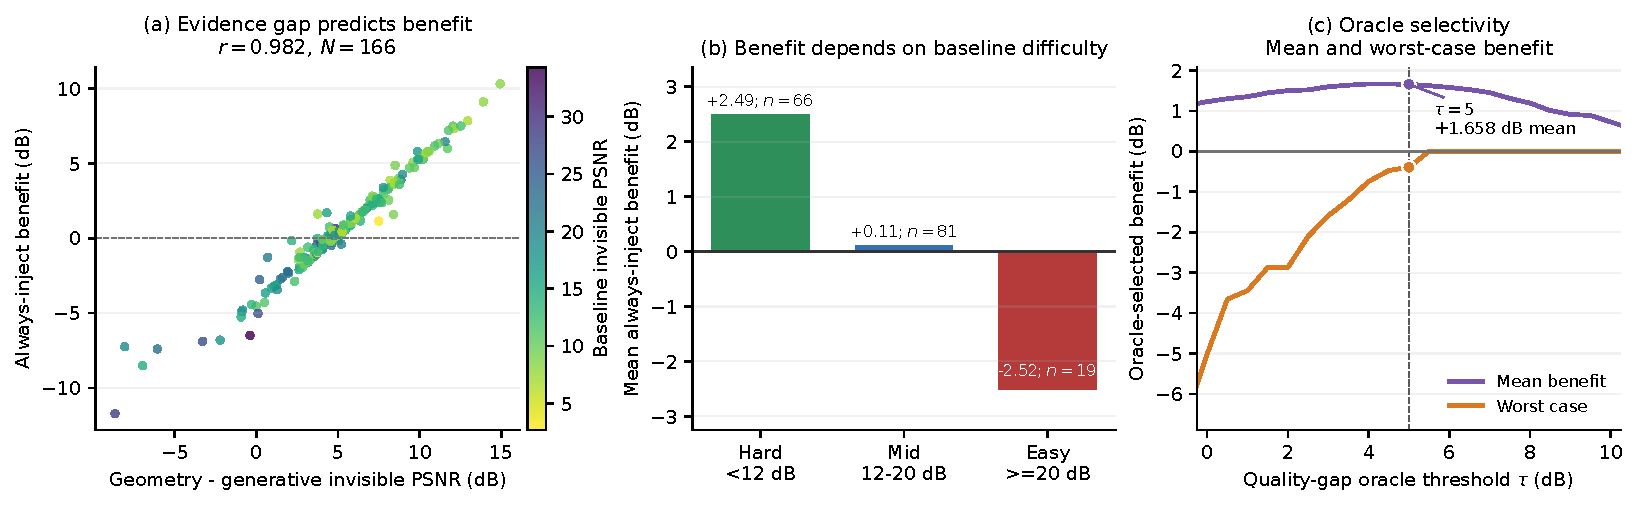
\includegraphics[width=\textwidth]{fig_mechanism_combined.pdf}
\caption{Mechanism evidence derived from released scene JSONs ($N=166$). (a) Each
point is one scene: the Flash3D-evidence minus Gen3R invisible PSNR gap predicts
actual always-inject benefit ($r=0.982$); color denotes baseline difficulty. (b)
The same benefit is positive for hard baselines ($+2.49$ dB), near zero for mid
cases ($+0.11$), and negative for easy cases ($-2.52$), with bucket counts shown.
(c) Sweeping the oracle-gap threshold exposes the mean/tail trade-off; markers
show the released default $\tau=5$ ($+1.658$ dB mean, $-0.393$ dB worst). Together
the panels show why evidence helps selectively rather than universally.}
\label{fig:mechanism}
\end{figure*}

The correlation remains .985, .980, .983, .984, and .982 at N=16, 92, 129, 149,
and 166; the N=166 bootstrap CI is $[.973,.990]$. This scale stability supports a
mechanism rather than a small-sample association.

\subsection{Cross-Dataset Mechanism Transfer}
\label{sec:acid}
We apply the mechanism without retuning to converted ACID aerial trajectories.
This is a diagnostic, not an official leaderboard result. The released E-215 aggregate contains
8 valid scenes: always injection averages $-0.443$ dB and wins 3/8 scenes.
This is failed zero-shot transfer and evidence that selectivity is
dataset-dependent, not mechanism success; no per-bucket ACID claim is released.

\subsection{Qualitative Successes and Failures}
Figure~\ref{fig:teaser} isolates three obvious released recoveries and an
injected failure that motivates a future fallback; it does not show a routing
decision. Figure~\ref{fig:diagnostic} provides sequence-level context.
\begin{figure*}[t]
\centering
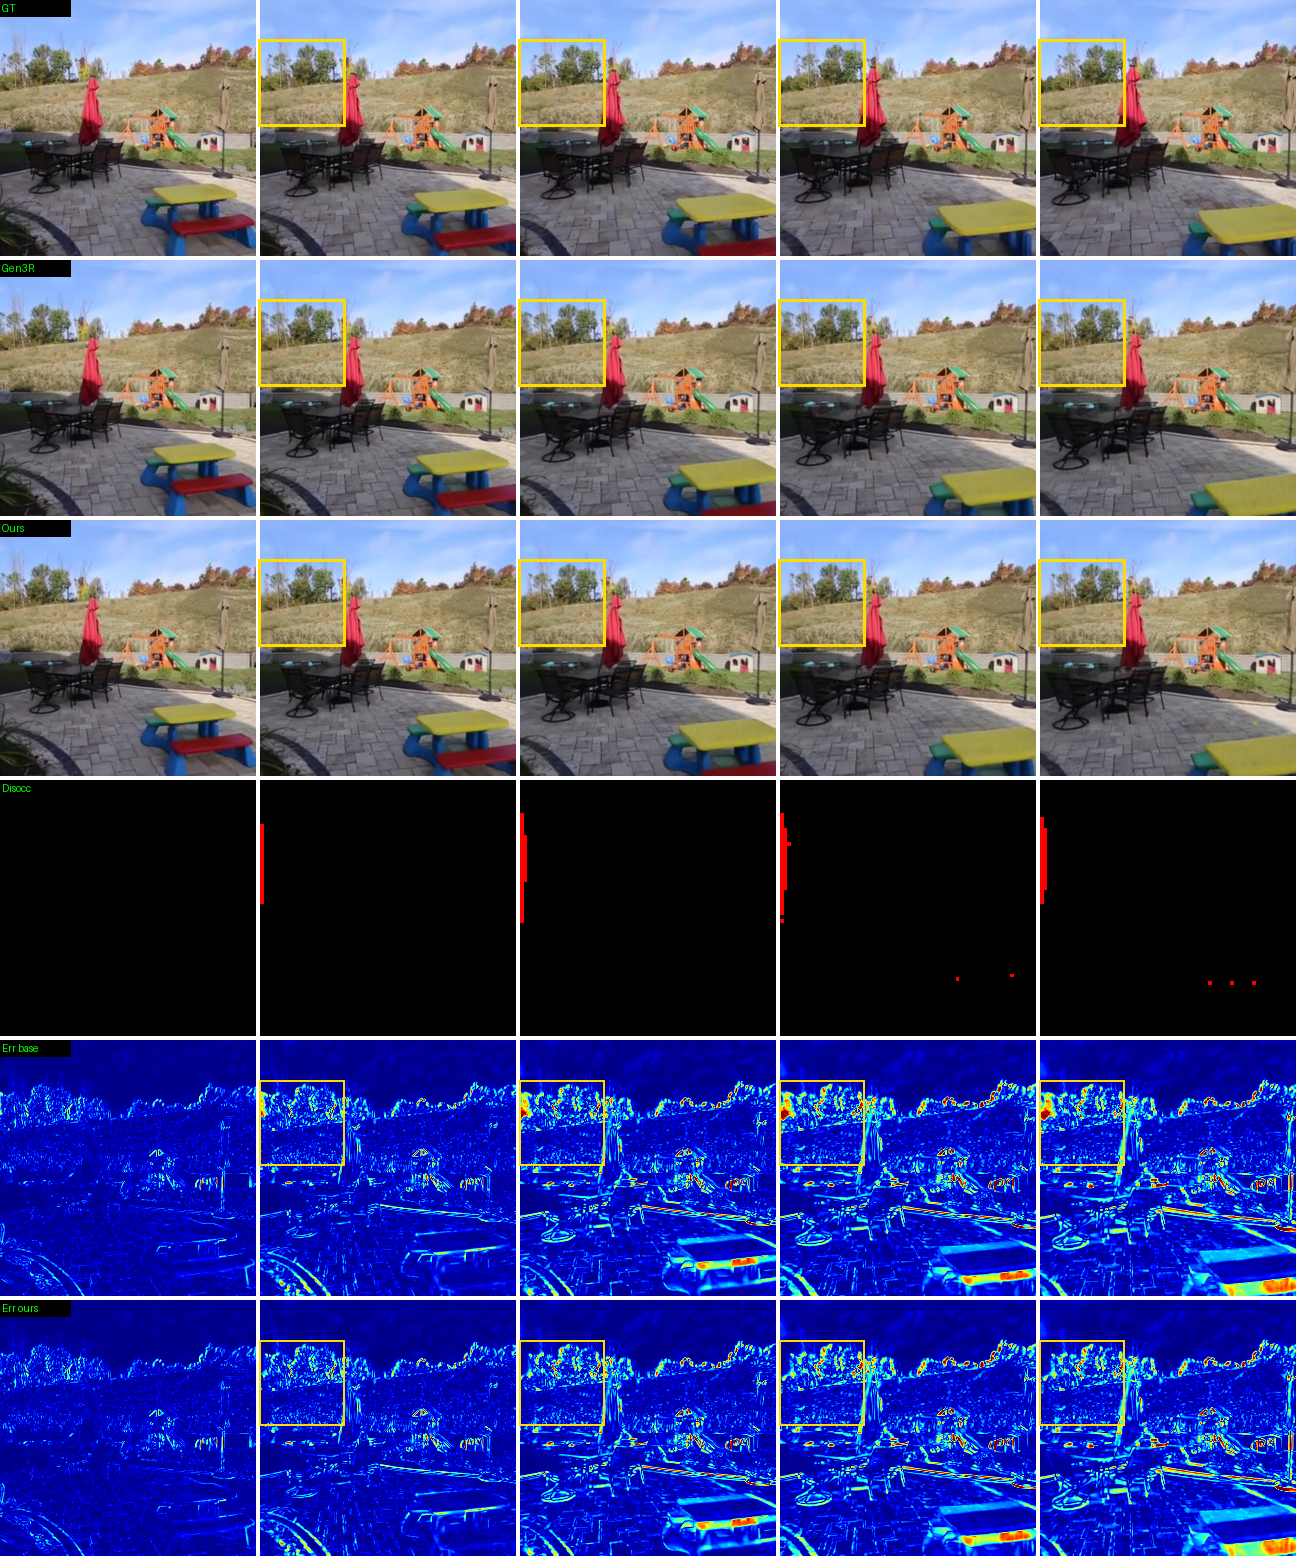
\includegraphics[width=\textwidth]{panel_success_boxed.png}
\caption{Successful long-sequence component diagnostic. Columns are successive
target views. Rows are GT, Gen3R, injected candidate, disocclusion mask, Gen3R
error, and candidate error. The same yellow ROI is used across corresponding
image and error rows; brighter error denotes larger residual. Error decreases in
the newly revealed patio while content outside the ROI is unchanged.}
\label{fig:diagnostic}
\end{figure*}

\begin{figure*}[t]
\centering
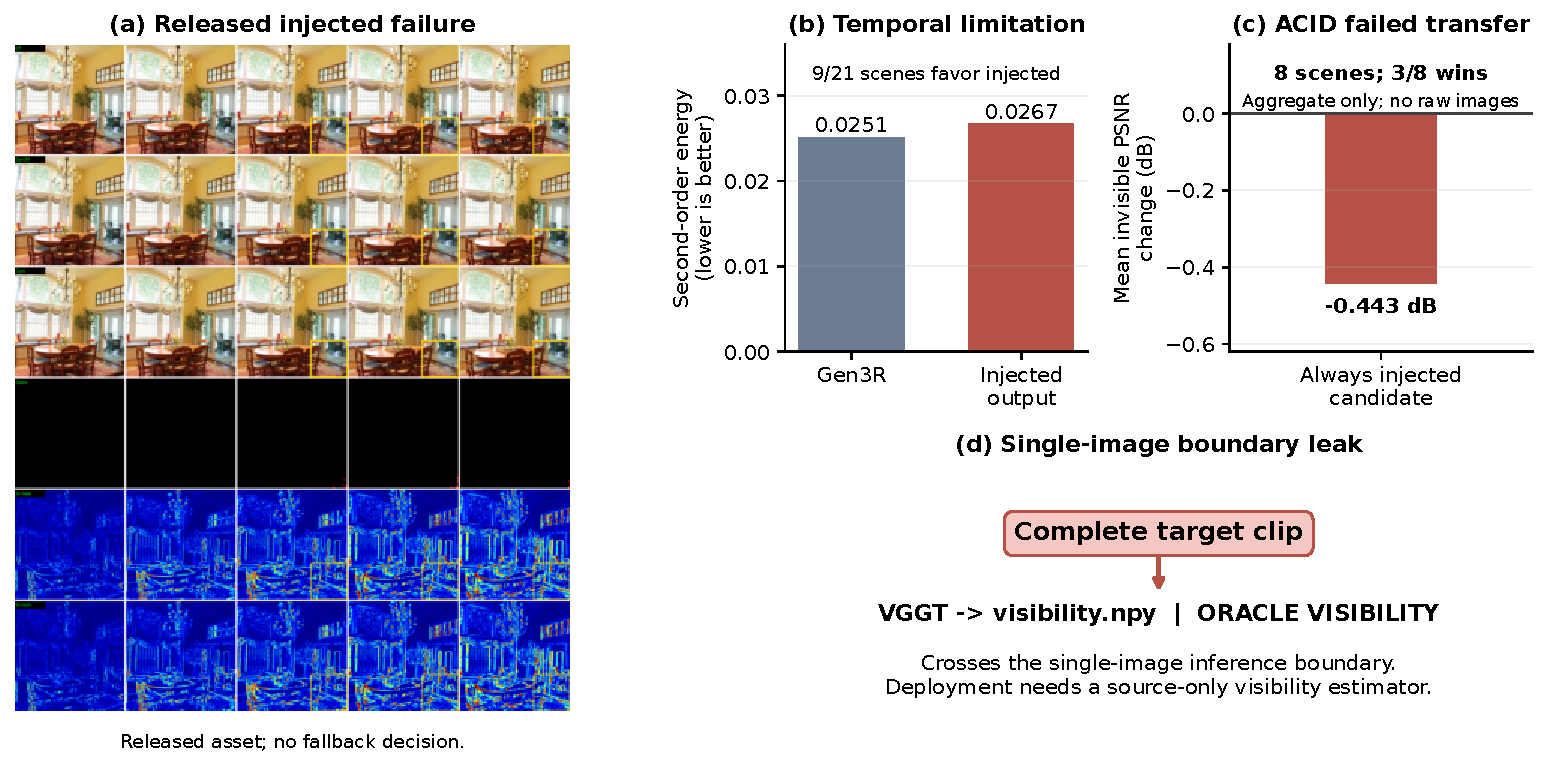
\includegraphics[width=\textwidth]{fig_failures_limitations.pdf}
\caption{Failure and limitations summary. (a) The released injected candidate
fails; no fallback decision exists. (b) Second-order disocclusion energy is .0251
for Gen3R and .0267 for the injected output over 21 scenes, with 9/21 wins. (c)
ACID has 8 scenes, a $-0.443$ dB always-injected mean, and 3/8 wins; no raw ACID images
are shown. (d) The critical inference-boundary leak: VGGT consumes the
complete target clip to produce \texttt{visibility.npy}. Thus all current mask and
injection results are offline oracle-visibility diagnostics. Deployment requires
a source-only visibility estimator.}
\label{fig:failures}
\end{figure*}

\subsection{Published Positioning Only}
\begin{table*}[t]
\centering\small
\caption{Quoted published RealEstate10K positioning only; values are not
reproduced and no cross-protocol winner is marked. The two-view rows share the
official pixelSplat protocol; Flash3D rows share the official MINE protocol.
Exact split/index, resolution/crop, target definitions, LPIPS backbone,
source/version/table, and checkpoint status are declared in
\texttt{../PROTOCOL.md}. None uses test-time optimization.}
\setlength{\tabcolsep}{9pt}
\begin{tabular}{lccrrr}
\toprule
Method & Views & Official target bucket & PSNR & SSIM & LPIPS-VGG \\
\midrule
pixelSplat~\cite{pixelsplat} & 2 & 3 interpolated & 26.09 & .863 & .136 \\
MVSplat~\cite{mvsplat} & 2 & 3 interpolated & 26.39 & .869 & .128 \\
DepthSplat-L~\cite{depthsplat} & 2 & 3 interpolated & 27.47 & .889 & .114 \\
\midrule
Flash3D~\cite{flash3d} & 1 & +5 & 28.46 & .899 & .100 \\
Flash3D~\cite{flash3d} & 1 & +10 & 25.94 & .857 & .133 \\
Flash3D~\cite{flash3d} & 1 & U[-30,30] & 24.93 & .833 & .160 \\
\bottomrule
\end{tabular}
\label{tab:positioning}
\end{table*}
The exact quoted sources are Flash3D arXiv:2406.04343v2 Table 2;
pixelSplat's camera-ready/retrained README (arXiv:2312.12337v4 Table 1
agrees; checkpoint N/A); arXiv:2403.14627v2 Table 1; checkpoint N/A for
MVSplat; and arXiv:2410.13862v3 Table 6; checkpoint N/A for DepthSplat-L.
The Flash3D rows are the official $+5$, $+10$, and U[-30,30] buckets; full
protocol details remain in \texttt{../PROTOCOL.md}.

\section{Limitations}
The complete target clip is consumed by VGGT to produce \texttt{visibility.npy};
this oracle visibility crosses the single-image inference boundary. A deployable
system needs a source-only visibility estimator that predicts target visibility
from the source image and requested camera alone, plus a source-observable
selector. Neither is released or evaluated. The released scene-level policies use
target-GT quality probes and are oracle analyses. The latent mask is exact, but
final visible RGB invariance is not guaranteed because the VAE/decoder may mix
spatially; the direct 16-scene change is $+0.016$ dB. Large-scale equal visible
values are a construction assumption, not an independent measurement. Flash3D
evidence is a per-target component reference, not an official single-view reproduction. The teaser is constrained to released
GT/Gen3R/injected assets; missing input/Flash3D assets are a release limitation,
and this reviewer-visible exception permits the strongest honest teaser rather
than invented replacements. Finally, per-frame injection does not optimize temporal
consistency: second-order disocclusion energy is .0251 for Gen3R and .0267 for
ours over 21 scenes, with ours more stable in 9/21.

\section{Conclusion}
Under oracle visibility, geometry evidence helps when it is better than the
generative prior in newly revealed regions. The exact latent bypass and measured
RGB behavior isolate the injection mechanism, while oracle selectivity quantifies
a future fallback opportunity. Source-only visibility and selection remain
necessary before this diagnostic can become deployable single-view inference.

{\small
\bibliographystyle{plain}
\bibliography{refs}
}
\end{document}
